\chapter{A generic representation for orthographic structure in texts written by children}\label{ch:adelaideherci14}
\chapterauthor[1]{Adelaide H.P. Silva}
\chapterauthor[1]{Fabiano Silva}
\chapterauthor[1]{Wanderlan Carvalho}
\chapterauthor[1]{Lourenço Chacon}
\begin{affils}
\chapteraffil[1]{UFPR/DELLIN/LIAMF/CNPq}
\end{affils}

%%%%%%%%%%%%%%%%%%%%%%%%%%%%%%%%%%%%%%%%%%%%%%%%%%%%%%%%%%%%%%%%%%%%%%
\section{Introduction}
Even though spelling is taken as a parameter to evaluate whether an individual is literate or not, Brazilian students from 3\textsuperscript{rd} and 5\textsuperscript{th} grade of Elementary School achieve a low performance in tests that verify their knowledge of the Brazilian Portuguese spelling. The last edition of the National Literacy Exam, held in 2016, points that 34\% of the children evaluated did not achieve the expected scores for literate students. So, we designed a software system, \emph{Scriba}, that generates orthographic forms such as the ones found in texts written by 3\textsuperscript{rd} and 5\textsuperscript{th} grade children. We expect Scriba to offer subsidies for teachers to understand the hypotheses underlying the forms that deviate from standard orthographic rules. We also expect that Scriba can provide teachers resources to evaluate whether or not the ``errors'' fit a given grade.

For the system to learn how to produce deviant forms and simulate the ``errors'', the first step was the analysis of data to classify ``errors'' and to detect patterns that group them following criteria such as type of ``error'' and school grade.
Concomitantly to grouping and classifying the ``errors'', we propose a generic representation for orthographic structure in texts written by children, so that Scriba can help understanding the hypotheses that lead to deviations.

Both tasks -- ``errors'' classification and the elaboration of a representation for orthographic structure -- are based on a corpus of 168 texts, containing 45561 words.
We assumed the orthographic words as the unities of analysis because they are the domain in which the spelling deviations occur.
Furthermore, and considering the findings of \citet{Chacon2018}, we focus on the syllable, within the orthographic word. This is because the syllable allows us to observe relationships between graphemes, as well as to make predictions about these relationships and the sounds they annotate. In the following sections we present and discuss
the representation we elaborated to annotate the internal structure of orthographic words.

%%%%%%%%%%%%%%%%%%%%%%%%%%%%%%%%%%%%%%%%%%%%%%%%%%%%%%%%%%%%%%%%%%%%%%
\section{Criteria for making the labels}

Predictions are at the heart of the algorithm for Scriba. In order to be able to predict the ``errors'', their nature, the graphemes involved in them and if they occur within the limits of a syllable, or extrapolate them, we proposed a set of labels, still as part of the initial process of formal representation of existing elements in a spelling word. The tags include: syllabic bondaries inside spelling words; internal structure of syllables; placement of primary stress in words; stress degree; consonant class. Table \ref{tab_labels} presents the set of the labels.

\begin{table}[!ht]
\caption{Spelling word representation labels.}
\label{tab_labels}
\centering
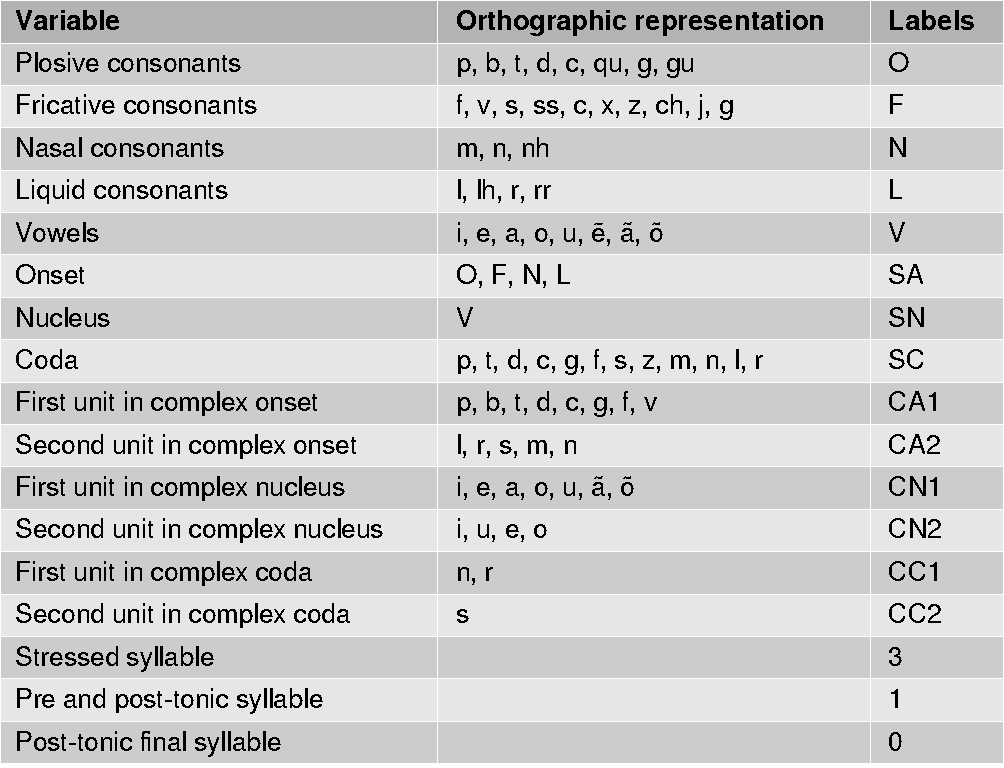
\includegraphics[width=0.9\textwidth]{imgs/adelaideherci14-labels.pdf}
\end{table}

As can be seen in Table \ref{tab_labels}, each variable is assigned a label. Here, labels attached to variables are based on Brazilian Portuguese, and that's the reason why some of them may seem weird at first sight. The variables cover: the type of segments, such as vowels and consonants and, within the set of consonants, subsets were established following the parameter \emph{manner of articulation}. The set of vowels gather oral and nasal sounds. Within each subset, or type of segment, consonants and vowels are associated to the possible graphemes that annotate them.

Variables also take into account the position of each unit within the syllable. Following the phonotactic constraints in Brazilian Portuguese, as presented, e.g., by \citet{Collischonn1996}, we assume that only vowels can ocuppy syllable nucleus. We also assume that the subset of consonants that occur in syllable codas is smaller than the subset of consonnats that occur in syllable onset. Notice that there is also the prediction on the units that can occur in the second position in complex syllabic constituents and we assign a numerical index for the consonant to indicate whether it is the first or the second unit in a complex constituent. By doing so, we offer an internal representation for the syllables in Brazilian Portuguese (BP).

The prosodic structure of the word is captured by the labels by assigning stress levels to the syllables, such as predicted by \citet{Camara1970}. Thus, numerical index 3 is attributed to the syllable that carries the primary stress in the word. Numerical index 1 is attributed to pretonic and postonic syllables. In the case of the postonic syllables, index 1 applies only in cases where the syllable is not the last one in the word, i.e., in syllables that immediately follow the stressed one in proparoxytone words. Numerical index 0 is attributed to postonic syllables that are also the last ones in the word. Numerical index 2, in turn, is assigned to secondary stress, i.e,. in cases where the primary stress of the basis turns into the secondary one by means of morphological operations, such as derivations, e.g., ``café'' - ``cafezinho'' (coffee and its corresponding diminutive form). In ``cafezinho'', the suffix ``-inho'' is stressed, and carries the primary stress of the form, because the most prominence domain lays at the rightmost position in BP. As a consequence, the syllable ``fe'' loses intensity and turns out to be the second more prominent syllable in the word, thus carrying the secondary stress.

It is worth adding that the labels allow us to better capture and understand how the units relate to each other and predict possible sequences, as well as the sequences of units that violate constraints of well-formedness, such as sequences of graphemes that write sound sequences that do not obey the sonority scale, and also sequences of graphemes that annotate randomized sequences of consonants, with no intervenient vowels. Thus, e.g., the labels allow us to predict that BP has a syllable such as ``por'', in words like ``porta'' (door), but has no syllable with ``rt''. This prediction has an obvious consequence for machine learning tasks: BP native speakers know the internal structure of the syllables in the language, so they perform quite well in establishing syllable boundaries. But the same is not true for a machine, that does not know the internal structure of BP syllables. So, considering that the syllable is the domain where ``errors'' apply, it is necessary to teach the machine the internal structure of syllables in the language. As the labels are machine-readable, the system can learn the internal structure of syllables.

It is worth mentioning that the labels do not take into account the number of the syllalbles within the word, because \citet{Chacon2018} did not observe possible influences of this variable on children's spelling ``errors''. But the information can be added to the labels, if it's necessary some time, since we plan to put aditional data into the corpus.

%%%%%%%%%%%%%%%%%%%%%%%%%%%%%%%%%%%%%%%%%%%%%%%%%%%%%%%%%%%%%%%%%%%%%%
\section{Application of the labels to words}
Table \ref{tab_examples} displays a set of examples of labeled data from the corpus of written texts by children. Data are organized according to number of syllables within the word and primary stress placement. In Table \ref{tab_examples}, segments boundaries are indicated by parentheses and syllables boundaries are indicated by brackets. This strategy for indicating boundaries was adopted in the light of the considerations presented in section 2 concerning machine learning and the need to teach the system which syllable structures are possible in BP.

\begin{table}[!ht]
\caption{Labeling examples for words in the dataset.}
\label{tab_examples}
\centering
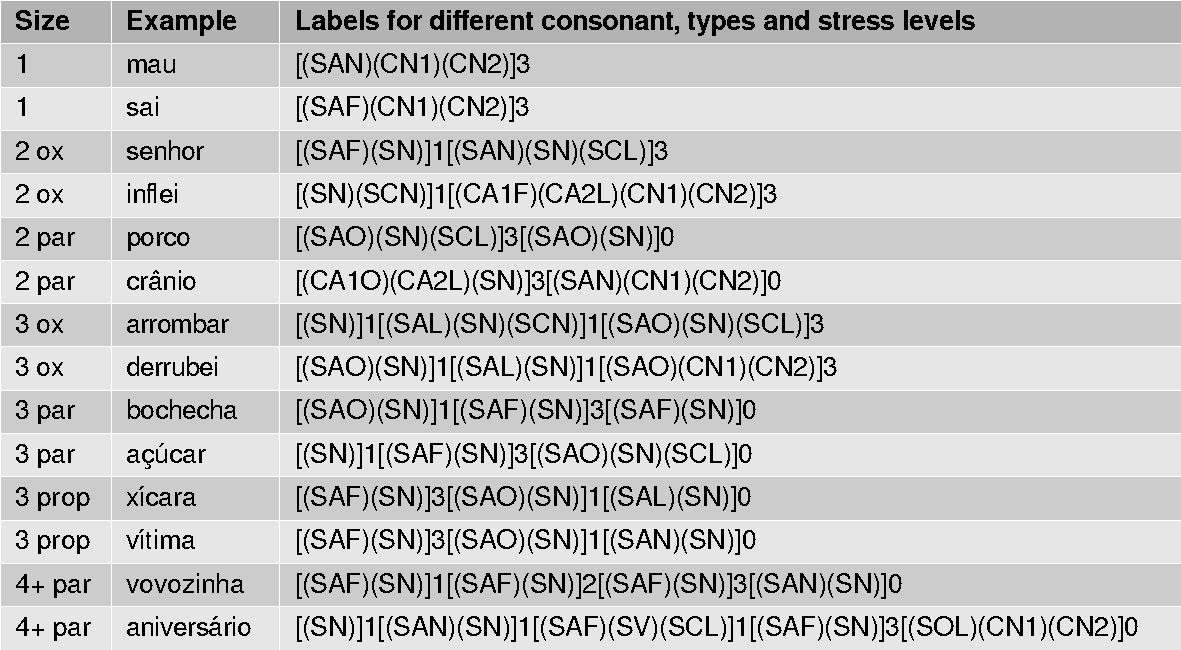
\includegraphics[width=0.9\textwidth]{imgs/adelaideherci14-examples.pdf}
\end{table}

The numerical stress indices (0, 1, 2, 3) follow the proposal of \citet{Camara1970}. `S', at the beginning of the label sequence, within a syllable, marks Onset or Simple Nucleus, while `C', preceding these tags, marks complex syllabic constituents. In the case of Complex Codas, we have a CC sequence. In the case of complex syllabic constituents, the proposed tag system makes it possible to identify whether a consonant is the first or second within the sequence. For diphthongs, we follow  \citet{Collischonn1996} proposal, which predicts the existence of a complex syllabic nucleus in BP. To clarify the labels interpretation, take the notation for the word ``vovozinha'', a paroxytone with four syllables, in:
\begin{center}
[(SAF)(SN)]1[(SAF)(SN)]2[(SAF)(SN)]3[(SAN)(SN)]0
\end{center}
from left to right: the first syllable has two units, being the first one a fricative consonant F occuring in a simple S onset A. It is followed by a simple S nucleus N and has stress level 1, i.e., it is pretonic. The second syllable has also two units. Like in the preceding syllable, the first unit is a fricative consonant, followed by a vowel. But the second syllable is assigned stress level 2, because it carries the former information on the primary stress placement in the word ``vovó'' before a derivational process applied. The third syllable has also two units, out of which the first one is a fricative consonant and the second one, a vowel. This is the stressed syllable in the word, and the primary stress is informed by the stress level 3. Finally, the last syllable has a nasal N consonant in simple S onset A, followed by a single vowel in the nucleus. The last syllable is assigned level 0, since it is the postonic one and, consequently, the less prominent syllable within the word.

%%%%%%%%%%%%%%%%%%%%%%%%%%%%%%%%%%%%%%%%%%%%%%%%%%%%%%%%%%%%%%%%%%%%%%
\section {Final remarks}
The labels we propose here are machine readable and correspond to some abstraction departing from real data. As a consequence, they can provide teachers a way to understand the hypotheses children formulate when they make spelling ``errors''. And the machine can learn to simulate such errors. Nevertheless, the labels do not specify which vowel occurs in syllable nucleus. According to Table \ref{tab_labels}, seven oral vowels and five nasal ones can be the nucleus of syllables in BP. There are ``errors'' that encompass vowel quality, such as ``rechunchuda'' (for ``rechonchuda'', chubby) or ``ispludiu'' (for ``explodiu'', it exploded). One possible way to solve the problem is to propose additional labels that deal with different opening degrees of aperture, because this is the parameter related to jaw opening that differentiates between /\textipa{O}/, as in ``vovó'' (grandma) and /o/, as in ``vovô'' (grandpa). Besides that, vowels also differentiate according to the place of the vocal tract they are articulated in: the palate, the velum or an intermediate point.

To accommodate these information in our labels, we propose four degrees of aperture, expressed by numerical indices that follow the labels `fr', i.e., \emph{frontal}, for vowels articulated in the hard palate; `ct', or \emph{central}, for vowels articulated in an intermediate place between the hard palate and the velum, and `pt', or \emph{posterior}, for vowels articulated in the velum. Then, we can rewrite the ``vovozinha'' example as in:
\begin{center}
[(SAF)(SNpt2)]1[(SAF)(SNpt3)]2[(SAF)(SNfr1)]3[(SAN)(SNct)]0
\end{center}

By doing so, we can properly differentiate between the vowels in the first and second syllables (from left to right) in the word. The next step, then, is make the system learn the labels and, departing from them, learn to produce non deviant orthographic forms for a set of words, as well as the deviant corresponding ones.

%%%%%%%%%%%%%%%%%%%%%%%%%%%%%%%%%%%%%%%%%%%%%%%%%%%%%%%%%%%%%%%%%%%%%%
\bibliographystyle{plainnat}
\bibliography{adelaideherci14.bib}

